\documentclass{article}
\usepackage{blindtext}
\usepackage{titlesec}
\usepackage{listings}
\usepackage{geometry}
\usepackage{mathtools}
\usepackage[utf8]{inputenc}
\usepackage{siunitx}
\usepackage{soul}
\usepackage{enumitem}

\geometry{
 a4paper,
 total={170mm,257mm},
 left=20mm,
 top=20mm,
 }


\title{Digital Systems Design Report 1}

\author{
  Pranav Malhotra, CID:\num{00823617}\\\\
  Dada Oluwatomisin, CID:\num{00846141}\\
}
\date{29th January 2016}

\begin{document}
\maketitle

\newpage
\tableofcontents

\newpage
\section{Aims}
\paragraph{}
We have the following aims that we hope to achieve by completing Task \num{1} and Task \num{2} of the Digital System Design Coursework.
\begin{enumerate}
  \item Get familiar with the design of a NIOS II processor and the design choices that impact the system’s performance.
  \item Use industry standard tools such as Quartus II and analyse compilation reports and assess feasibility of design.
  \item Use industry standard tools such as Nios II Eclipse and analyse project size and resource allocations; conduct application profiling and understand linker files and .map files. 
  \item Analyse performance of program in terms of accuracy, speed and amount of resources used.
\end{enumerate}

\newpage
\section{System on Programmable Chip Components}
\paragraph{}
In this section, we will be discussing the components that our system consists of.
\paragraph{}
We will use a \num{50}Mhz clock generated on the Cyclone III Chip to drive all parts of our Nios II processor. A processor clocked at \num{50}Mhz is significantly slower than modern processors, such as Intel E\num{5}-\num{1620}V\num{2}, which are clocked at \num{3.7}GHz\cite{intel}. However, the NIOS II processor provides the advantage of being a soft processor. We can add and remove complexity as we like. The NIOS II processor also allows us to add custom instructions that enable hardware acceleration. This is ideal for our task.
\paragraph{}
On-chip memory is the highest throughput, lowest latency memory possible in an FPGA-based embedded system. It typically has a latency of only one clock cycle\cite{highest_throughput}. For task \num{1} and task \num{2}, we use on-chip memory to store our program, initialization data, stack and heap. However, On-Chip Memory is more occasionally used for:
\begin{itemize}
  \item Separate exception stack for use only while handling interrupts 
  \item Fast data buffers
  \item Fast sections of code
  \item Fast interrupt handler
  \item Critical loop
  \item Constant access time that is guaranteed not to have arbitration delays\cite{on-chip_memory}
\end{itemize}
\paragraph{}
During the tutorial, we included an instruction cache in our system. Caches are added to streamline instruction fetches from external memory locations. Because memory accesses in most computer programs display some sort of temporal or spatial locality, fetching instructions from multiple memory locations and storing them in locations near the processor will significantly reduce latency. Because caches are also stored on on-chip memory, it does not make much sense to add an instruction cache to our system at this point. Instruction caches will come in handy in future tasks should we load our program and initialisation data onto the external SDRAM.
\paragraph{}
The interval timer is added to allow us to measure our program’s performance using the times(NULL) command. We could keep implement a counter in software, however, this would cause a structural hazard as we will be using the Arithmetic Logic Unit (ALU) of the processor to maintain our counter instead of having dedicated hardware to do so. The interval timer core generates an IRQ whenever the internal counter reaches zero. This is an interrupt request (IRQ) that we have to handle. The Nios II HAL interprets low IRQ values as higher priority. The timer component must have the highest IRQ priority to maintain the accuracy of the system clock tick.\\

\newpage
\section{Memory Allocation on System}
\paragraph{}
A major problem that we were facing while completing task \num{2} was that our program would not fit onto our NIOS II Processor. We then looked at the .map file that gave us the breakdown of our memory usage. Below is a short description of each data segment and what they are used for.
\begin{itemize}
    \item The .data segment contains any global or static variables which have a pre-defined value and can be modified. That is any variables that are not defined within a function (and thus can be accessed from anywhere) or are defined in a function but are defined as static so they retain their value across subsequent calls.
    \item The .bss segment, also known as uninitialized data, is usually adjacent to the data segment. The BSS segment contains all global variables and static variables that are initialized to zero or do not have explicit initialization in source code.
    \item The .rodata segment is a read-only data segment that contains static constants rather than variables.
    \item The .text segment contains the program's executable instructions. This data segment is read-only on many architectures to prevent a program from accidentally modifying instructions.\cite{wiki}  
\end{itemize}
\paragraph{}
The gcvt instruction requires numerous libraries to be imported. This significantly increases the program size. Using the printf function, we were able to reduce our program size and evaluate the function for test case 2. Studying .map files gave us clearer understanding of the memory layout of a C program which is bound to come in handy in the upcoming tasks. 

\newpage
\section{Implementations of Function}
For task 2, we had to evaluate the expression: 
\begin{equation}
     \sum_{i=1}^{N} x_i + x_i^2 
\end{equation} 
We evaluated the expression over the provided vector with many different algorithms which are explained below.

\subsection{Analytic Algorithm}
\paragraph{}
To evaluate the equation, we formed a closed form expression that takes advantage of the regular nature of the test cases. Our algorithm only uses the step size and the size of the vector to compute the answer. We expect the analytic algorithm to have the best performance as it does not access the vector x. This algorithm, however is not representative of the computational complexity that is required for the future tasks for two main reasons. Firstly, our algorithm will not work on any arbitrary vector x. Secondly, the equation in the following tasks does not have a closed form expression.\\\\
\lstset{
language=C,
showspaces=false,
showstringspaces=false,
}         

\begin{lstlisting}[frame=single]
float sumVectorAnalytic(float s, float M){
	return (s*(M/2))*(M-1)+(s*(M-1))*(s*M)*(2*(M-1)+1)/6;
}
\end{lstlisting}

\subsection{Iterative Algorithm}
\paragraph{}
The iterative algorithm is more representative of the approach we will use to complete the future tasks. A for loop runs through the vector x and evaluates the equation, accumulating the result in the variable sum. While storing our vector x, we can either store the values as single-precision floating points (float) or as double-precision floating points (double). A double will require twice as much space as a float, however, it will give us greater precision. The discrepancy in precision comes from the fact that when we conduct floating point additions, we require the exponents of the two numbers to be the same. To illustrate the cause of the error, we shall add \num{10000000} to \num{0.5}.
\\\\
We first write the numbers in their scientific notations:
\begin{equation}
    10,000,000 \xrightarrow[]{in scientific notation} 1.0011000100101101 * 2^{23}
\end{equation}
\begin{equation}
    0.5 \xrightarrow[]{in scientific notation} 1.0 * 2^{-1}   
\end{equation} 
\\\\
Next, we ensure that radix of the smaller number is shifted to ensure that both the numbers have the same exponent. Then, we perform the addition.\\\\
\centerline{
\begin{tabular}{ccccccccccccccccccccccccc}
    & 0 & 0 & 1 & 1 & 0 & 0 & 0 & 1 & 0 & 0 & 1 & 0 & 1 & 1 & 0 & 1 & 0 & 0 & 0 & 0 & 0 & 0 & 0 & 0 \\
+   & 0 & 0 & 0 & 0 & 0 & 0 & 0 & 0 & 0 & 0 & 0 & 0 & 0 & 0 & 0 & 0 & 0 & 0 & 0 & 0 & 0 & 0 & 0 & 1 \\
    \hline
    & 0 & 0 & 1 & 1 & 0 & 0 & 0 & 1 & 0 & 0 & 1 & 0 & 1 & 1 & 0 & 1 & 0 & 0 & 0 & 0 & 0 & 0 & 0 & 1 \\
\end{tabular}
}

\paragraph{}
This addition returns a mantissa that is \num{24} bits long. However the single-precision floating point representation only allows us to have a \num{23} bit mantissa. This means our result will be truncated and the last bit is ignored; the result is \num{10000000}. We notice that, adding two numbers that have an exponent that differ by more than \num{23} will result in effectively adding zero to our larger number. Floating point multiplications will cause similar rounding errors. Thus, we have to carefully plan the trade off between precision and complexity of our program, both in terms of computational time and memory usage. It is important to note that MATLAB, by default, stores all values as uses double-precision floating-points.
\paragraph{}
Below are two algorithms that implement the addition using floating points and doubles respectively. Their efficiency is discussed in the next section of this report.

\subsubsection {sumVectorFloat()}
\begin{lstlisting}[frame=single]
float sumVectorFloat()
{
	int i;
	float sum = 0;
	for(i=0; i<N; i++)
		sum += numbers[i]*(1+numbers[i]);
	return sum;
}
\end{lstlisting}

\subsubsection {sumVectorDouble()}
\begin{lstlisting}[frame=single]
double sumVectorDouble()
{
	int i;
	double sum = 0;
	for(i=0; i<N; i++)
		sum += numbers[i]*(1+numbers[i]);
	return sum;
}
\end{lstlisting}

\newpage
\section{Performance of Computation}
\subsection{Analytic Algorithm}
\paragraph{}
The analytic algorithm gives us the best performance. It has a time complexity of $O(1)$, a space complexity of $O(1)$ and the returns the same result as MATLAB. However, as stated above, the applications of an analytic algorithm are highly limited.
\subsection{Iterative Algorithm}
We tested the two iterative functions and obtained the following data.
\begin{figure}[h]
    \centering
    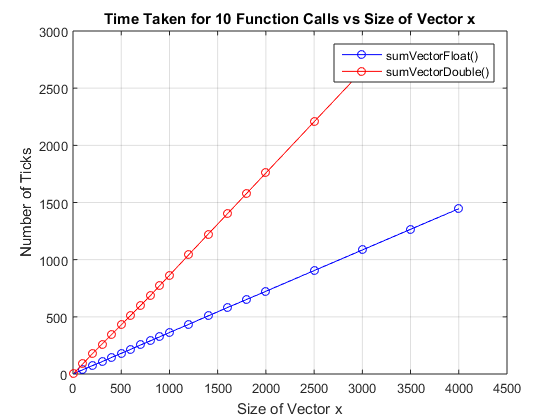
\includegraphics[scale=0.6]{EfficiencyOfFunctions}
\end{figure}
\paragraph{}
It is clear that the time taken for both functions increases linearly with the size of vector x. This is expected as the algorithm runs through the array once and thus has a complexity of $O(n)$. There is however a difference between the gradient of the two graphs. The difference arises from the fact that operations on double-precision floating points take significantly longer than operations on single-precision floating points.
\begin{figure}[h]
    \centering
    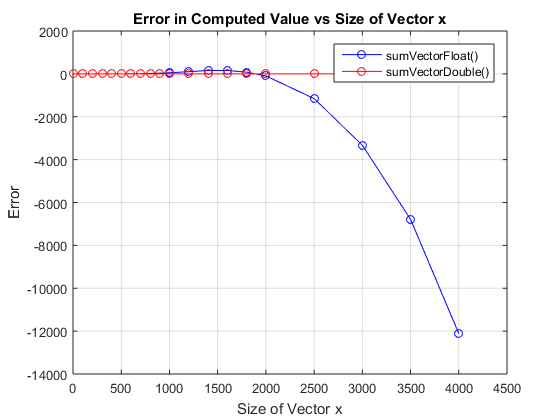
\includegraphics[scale=0.6]{ErrorOfFunctions}
\end{figure}
\paragraph{}
Comparing the two functions based on their precision, we see that as size of the vector increases, the function sumVectorFloat() returns a value with an error that grows exponentially. The error is introduced because of the truncation errors when adding floating-point numbers that have exponents that differ by more than 23. There are also errors that occur in sumVectorDouble() however these are due to the fact that we are using truncated libraries and thus cannot print floating-points. Thus, rounding off errors occur when we cast a double into an integer while printing. Tables of data collect are provided in the appendix.  

\newpage
\section{Questions asked in Booklet}
\begin{enumerate}[align=left]
    \item Record the FPGA resources used by your baseline system (i.e. Total logic elements, Total	memory bits, Embedded Multiplier \num{9}-bit elements, and Total PLLs). 
    \begin{itemize}
        \item For our baseline system we used, \num{2313} logic elements, \num{192384} memory bits and \num{0} embedded multiplier \num{9}-bit elements or PLLs. 
    \end{itemize}
    \item How many resources does your system occupy on the FPGA? (for Task \num{2})
    \begin{itemize}
        \item For our system to be able to compute test case 2, we had to increase the on-chip memory. We provided \num{49152} bytes of on-chip memory. As such, our system used \num{2335} logic elements, \num{421824} memory bits and \num{0} embedded multiplier \num{9}-bit elements or PLLs.
    \end{itemize}
    \item Is your system able to evaluate the given function for all test cases? Why not?
    \begin{itemize}
        \item We were not able to evaluate the function for the third test case using the iterative algorithm. For the iterative algorithm, we have to first generate the vector and store it in memory. The Cyclone III FPGA chip has limited memory bits and thus, without using an external source of memory such as the SDRAM (available on the DEO board), we cannot generate a vector of size 255001.
        \item To generate a vector of floats of size 255001, we would need \num{102004} bytes of memory. We are limited to \num{49152} bytes of on-chip memory, some of which has to be used to store our program.
    \end{itemize}
    \item What is the size of your NIOS II application for different vector sizes and what is the maximum memory required?
    \begin{itemize}
        \item The size of our application does not change for different vector sizes. The reason for this was discussed in detail in the data segment section of the report. The vector is declared in the main function and thus is generated on the stack.
        \item Should we declare the vector x as a global variable, then the program size + initialization data size will change. Studying the .map files, it is clear that single-precision floating points occupy 4 bytes of memory, whereas double-precision floating points occury 8 bytes of memory.
    \end{itemize}
    \item Compare your results with MATLAB. Do your results agree? If not, why not?
    \begin{itemize}
        \item As discussed in section \num{5}, when we used double-precision floating points to evaluate the function, we obtained the same results as MATLAB. There was a discrepancy in results when we used single-precision floating points. This was due to the truncation and rounding errors. 
    \end{itemize}
    \item What is the time required to evaluate the sumVector() function for each test case?
    \begin{itemize}
        \item A graph showing the amount of time it take to evaluate both iterative functions is presented in section \num{5}. Detailed data can  be found in the form of a table in Appendix A.
    \end{itemize}
    \item The best design is the one that provides the least latency for the least possible resources. Where is your current design in that space?
    \begin{itemize}
        \item As stated in the coursework booklet, we need vector x to be stored as a single-precision floating point. Our tests have conclusively shown that a single-precision floating point representation will use half as many resources and will be faster, however the error grows exponentially with the size of the vector x. Thus, limited  by the coursework stipulations, our design trades off precision for an increase in speed. In addition, a single-precision floating point representation allows us to minimise resources on the FPGA.
    \end{itemize}
\end{enumerate}

\newpage
\section{Conclusion}
\paragraph{}
We achieved the aims that were set out at the start of the report. Firstly, we gained a deeper understanding of the basic building blocks of the NIOS II system, made smart design choices to minimise the resources required while maximising efficiency and are now able to understand compilation reports and assess feasibility of our designs. 
\paragraph{}
Secondly, we noticed some of limitations that the NIOS II system has with regards to printing floating-point numbers and also studied how fundamental operations such as single-precision and double-precision floating point additions and multiplications affect our final result. We also learnt the way that memory is allocated on the NIOS II processor by looking at .map files.
\paragraph{}
Lastly, we designed two algorithms to evaluate the result of the expression. We studied some of the limitations of an analytic algorithm and analysed the performance of our iterative algorithm with respect to latency, precision and memory. 

\newpage
\begin{thebibliography}{99}

\bibitem{intel} Intel® Xeon® Processor E5-1620 v2 (10M Cache, 3.70 GHz) Specifications. (n.d.). Retrieved January 29, 2016, from \url{ http://ark.intel.com/products/75779/Intel-Xeon-Processor-E5-1620-v2-10M-Cache-3_70-GHz}.

\bibitem{highest_throughput} Corporation, A. (2010). Memory System Design. Retrieved January 26, 2016, from \url{https://www.altera.com/content/dam/altera-www/global/en_US/pdfs/literature/hb/nios2/edh_ed51008.pdf}.

\bibitem{on-chip_memory} Corporation, A. (2011). . Using Tightly Coupled Memory with the Nios II Processor. Retrieved January 26, 2016, from \url{https://www.altera.com/content/dam/altera-www/global/en_US/pdfs/literature/tt/tt_nios2_tightly_coupled_memory_tutorial.pdf}.

\bibitem{wiki} Data Segment. (n.d.). Retrieved January 26, 2016, from \url{https://en.wikipedia.org/wiki/Data_segment}.

\end{thebibliography}


\newpage
\appendix
\section{Data Collected}
\begin{table}[h!]
\centering
\begin{tabular}{c|c|c|c|}
\cline{2-4}
 & \multicolumn{3}{c|}{sumVectorFloat()} \\ \hline
\multicolumn{1}{|l|}{Size of Vector x, N} & \multicolumn{1}{l|}{Time Taken, ticks} & \multicolumn{1}{l|}{Result of Computation, y} & \multicolumn{1}{l|}{Error in Computation} \\ \hline
\multicolumn{1}{|c|}{10} & 4 & 7 & 0 \\ \hline
\multicolumn{1}{|c|}{101} & 37 & 3888 & 0 \\ \hline
\multicolumn{1}{|c|}{201} & 73 & 28877 & 0 \\ \hline
\multicolumn{1}{|c|}{301} & 108 & 94965 & 0 \\ \hline
\multicolumn{1}{|c|}{401} & 145 & 222154 & 0 \\ \hline
\multicolumn{1}{|c|}{501} & 181 & 430442 & 0 \\ \hline
\multicolumn{1}{|c|}{601} & 217 & 739827 & 4 \\ \hline
\multicolumn{1}{|c|}{701} & 254 & 1170310 & 9 \\ \hline
\multicolumn{1}{|c|}{801} & 290 & 1741889 & 19 \\ \hline
\multicolumn{1}{|c|}{901} & 326 & 2474563 & 33 \\ \hline
\multicolumn{1}{|c|}{1001} & 363 & 3388333 & 52 \\ \hline
\multicolumn{1}{|c|}{1201} & 435 & 5839160 & 102 \\ \hline
\multicolumn{1}{|c|}{1401} & 508 & 9254379 & 160 \\ \hline
\multicolumn{1}{|c|}{1601} & 581 & 13794058 & 158 \\ \hline
\multicolumn{1}{|c|}{1801} & 652 & 19618214 & 79 \\ \hline
\multicolumn{1}{|c|}{2001} & 724 & 26886866 & -96 \\ \hline
\multicolumn{1}{|c|}{2501} & 905 & 52428368 & -1156 \\ \hline
\multicolumn{1}{|c|}{3001} & 1085 & 90498488 & -3333 \\ \hline
\multicolumn{1}{|c|}{3501} & 1266 & 143597392 & -6795 \\ \hline
\multicolumn{1}{|c|}{4001} & 1446 & 214225664 & -12124 \\ \hline
\end{tabular}
\caption{Data for sumVectorFloat()}
\end{table}

\begin{table}[h!]
\centering
\begin{tabular}{c|c|c|c|}
\cline{2-4}
 & \multicolumn{3}{c|}{sumVectorDouble()} \\ \hline
\multicolumn{1}{|l|}{Size of Vector x, N} & \multicolumn{1}{l|}{Time Taken, ticks} & \multicolumn{1}{l|}{Result of Computation, y} & \multicolumn{1}{l|}{Error in Computation} \\ \hline
\multicolumn{1}{|c|}{10} & 8 & 7 & 0 \\ \hline
\multicolumn{1}{|c|}{101} & 88 & 3888 & 0 \\ \hline
\multicolumn{1}{|c|}{201} & 177 & 28876 & 1 \\ \hline
\multicolumn{1}{|c|}{301} & 261 & 94965 & 0 \\ \hline
\multicolumn{1}{|c|}{401} & 345 & 222154 & 0 \\ \hline
\multicolumn{1}{|c|}{501} & 430 & 430442 & 0 \\ \hline
\multicolumn{1}{|c|}{601} & 515 & 739831 & 0 \\ \hline
\multicolumn{1}{|c|}{701} & 599 & 1170319 & 0 \\ \hline
\multicolumn{1}{|c|}{801} & 685 & 1741908 & 0 \\ \hline
\multicolumn{1}{|c|}{901} & 775 & 2474596 & 0 \\ \hline
\multicolumn{1}{|c|}{1001} & 864 & 3388384 & 1 \\ \hline
\multicolumn{1}{|c|}{1201} & 1044 & 5839261 & 1 \\ \hline
\multicolumn{1}{|c|}{1401} & 1223 & 9254538 & 1 \\ \hline
\multicolumn{1}{|c|}{1601} & 1401 & 13794215 & 1 \\ \hline
\multicolumn{1}{|c|}{1801} & 1580 & 19618292 & 1 \\ \hline
\multicolumn{1}{|c|}{2001} & 1759 & 26886769 & 1 \\ \hline
\multicolumn{1}{|c|}{2501} & 2207 & 52427212 & 0 \\ \hline
\multicolumn{1}{|c|}{3001} & 2654 & 90495155 & 0 \\ \hline
\end{tabular}
\caption{Data for sumVectorDouble()}
\end{table}

\end{document}


